\subsection{Deep Bi-Dense Network (DBDN\cite{DBDN})}
\begin{figure}
    \centering
    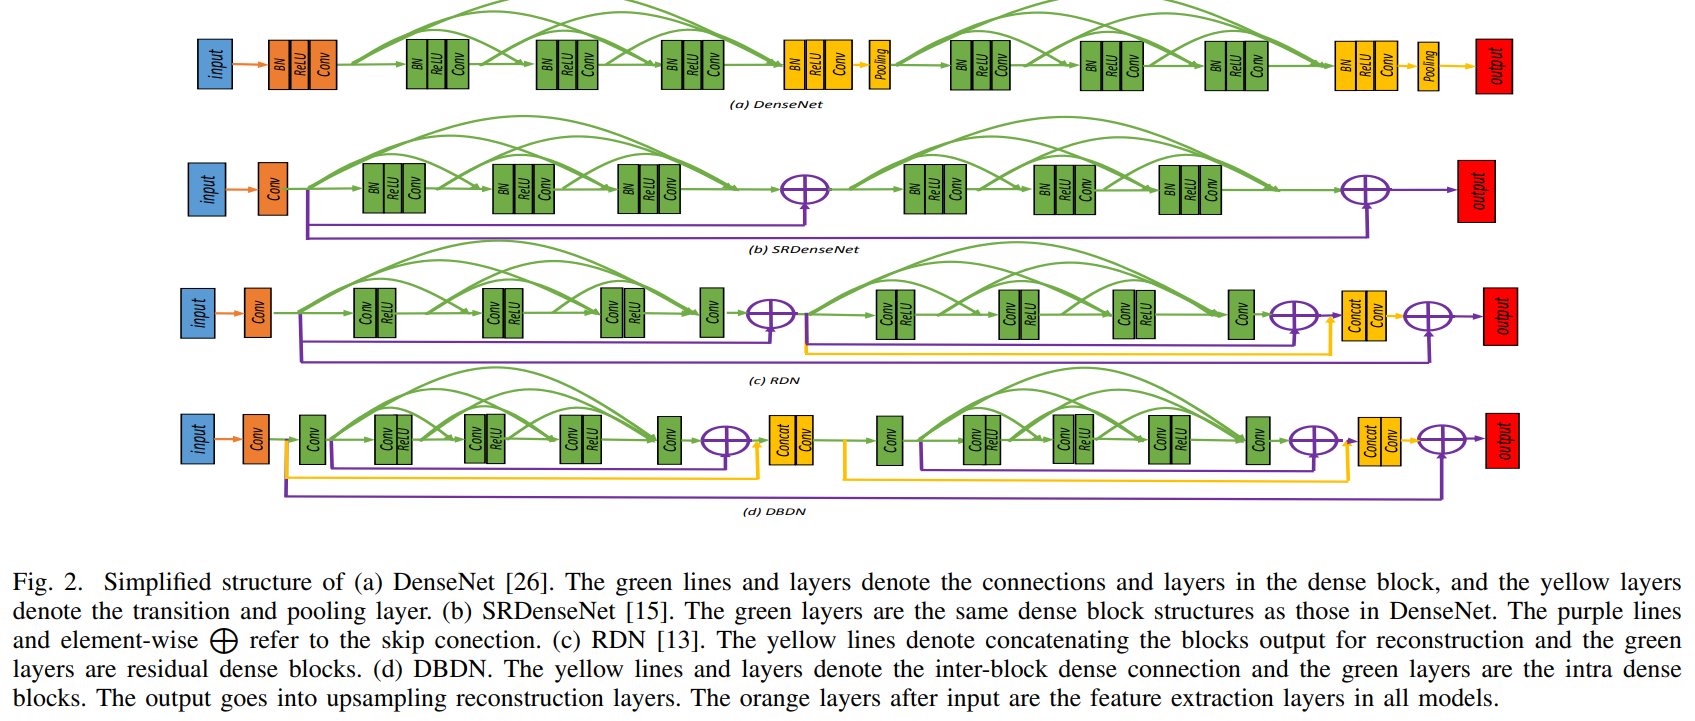
\includegraphics[width=\textwidth, keepaspectratio]{bidense-comparison.png}
    \caption{Comparison of different network that are using dense connection.}\label{dbdn:comparison}
\end{figure}

Skip connections allow to highlight one of the most important hyperparameter in deep network: the depth.

But in SR task an important aspect also is the use of features learned at the beginning of the network: therefore dense connection were adopted, moreover new architecture arose such as \textit{SRDenseNet} and \textit{RDN}.

All the previous mentioned architectures have a problem: the feature reusing is not really achieved as we can see from the \Cref{dbdn:comparison}.

Therefore the aim of Deep Bi-Dense Network (DBDN) is to be able to reuse the feature in the network thanks to dense connections used along the network and within each block.

\subsubsection{Architectures}
\begin{figure}
    \begin{subfigure}{\textwidth}
        \centering
        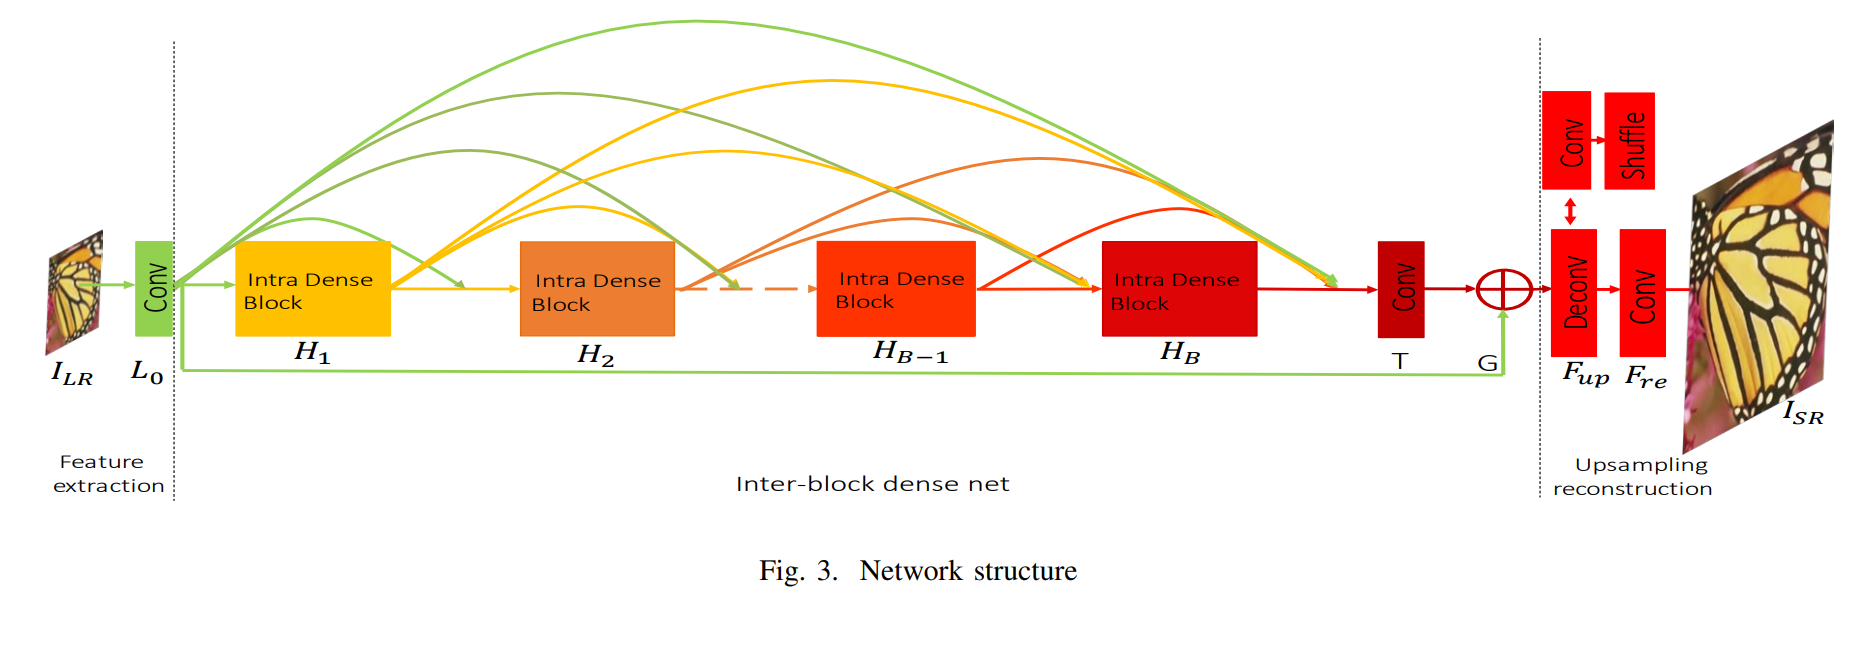
\includegraphics[width=\textwidth, keepaspectratio]{bidense-model.png}
        \caption{DBDN architecture.}\label{dbdn:architecture}            
    \end{subfigure}
    \begin{subfigure}{\textwidth}
        \centering
        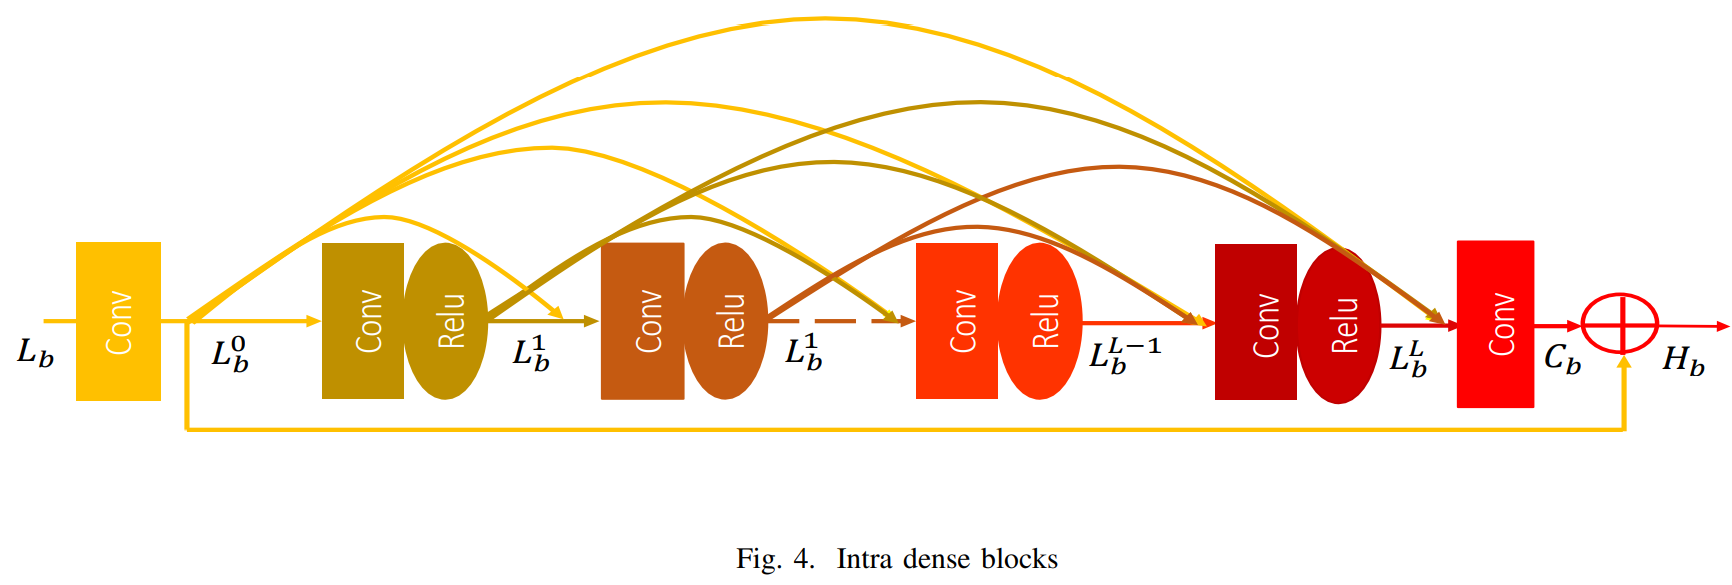
\includegraphics[width=\textwidth, keepaspectratio]{bidense-intra-dense-block.png}
        \caption{Intra dense block.}\label{dbdn:idb}   
    \end{subfigure}


\end{figure}

We can see from \Cref{dbdn:architecture} how features are reused: the features extracted by the single feature extraction convolution are processed by a sequence of \textbf{Intra dense block}.

The \textit{Intra dense block} contains at the beginning and at the end two convolutions which compress the input and the output channels (to $n_r$) and in the middle $L$ convolutions (with $n_g$ filters) and ReLUs, connected densely, process the compressed input.
The compressions are necessary due to the concatenation at the beginning of each intra dense block (\Cref{dbdn:architecture}) and at the end of each intra dense block (\Cref{dbdn:idb}):
\begin{itemize}
    \item $n_r \ast \textnormal{number of IDBs before}$.
    \item $n_r + L \ast n_g$ at the end of each IDB. 
\end{itemize}
The local residual learning allow the flowing of the gradients allowing a faster convergence.

Moreover a global skip connections is used in order to use low-frequency information from the LR image and allow the gradient to flow from the end to the beginning of the network.

The SR image is reconstructed using either deconvolution or sub-pixel convolution\cite{subpixel}

\subsubsection{Results}

\paragraph{Ablation studies on compression layer and inter-block dense connection}
\begin{figure}
    \centering
    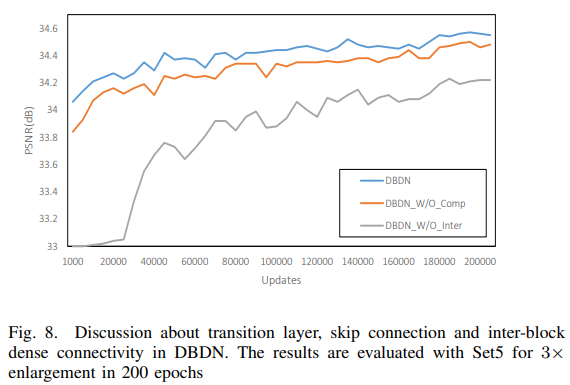
\includegraphics[width=\textwidth, keepaspectratio]{bidense-ablation-studies.png}
    \caption{Ablation studies on DBDN.}\label{dbdn-ablation-studies}
\end{figure}
From the \Cref{dbdn-ablation-studies} we can see that \textit{Intra dense-block connection} and \textit{compression layers} are important for achieving good results. 

\paragraph{Quantitative and qualitative results}
\begin{figure}
    \centering
    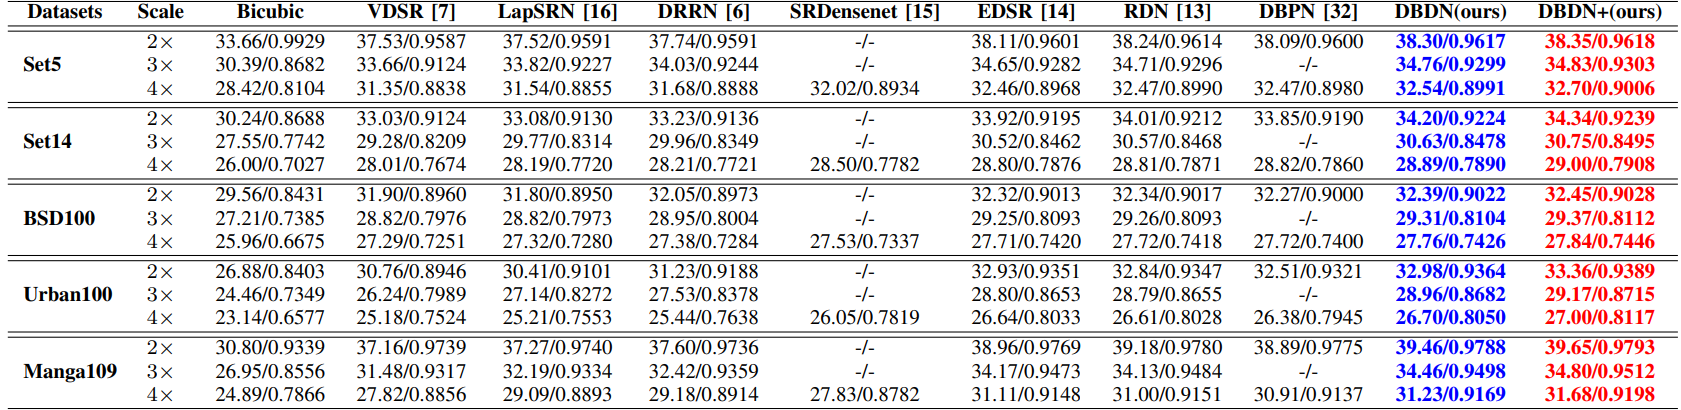
\includegraphics[width=\textwidth, keepaspectratio]{bidense-quantitative-results.png}
    \caption{Quantitative results on public benchmark. Red indicates best performance, blue indicates second best performance.}\label{dbdn:quantitative}
\end{figure}

\begin{figure}
    \centering
    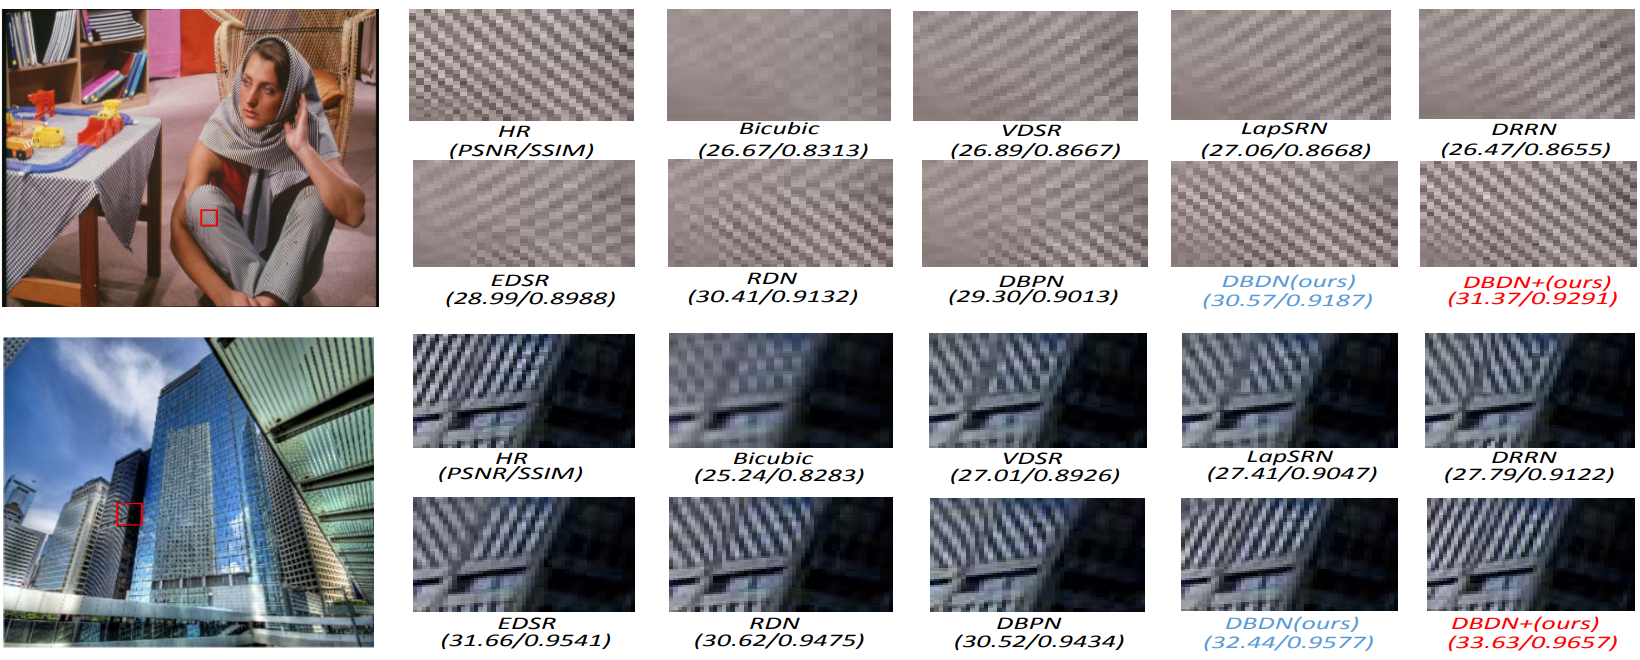
\includegraphics[width=\textwidth, keepaspectratio]{bidense-qualitative-results.png}
    \caption{Qualitative results of DBDN.}
\end{figure}
\begin{figure}
    \centering
    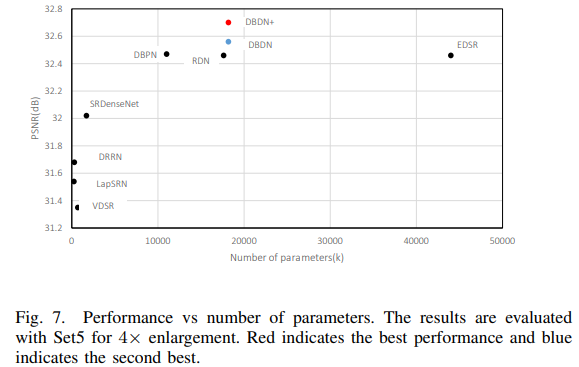
\includegraphics[width=\textwidth, keepaspectratio]{bidense-performace-paramters.png}
    \caption{Performance-Parameters study.}
\end{figure}

Thanks to the feature reusing the model perform better than state-of-the-art network maintaining the number of parameters low.